\documentclass[a4paper]{article}

\usepackage[english]{babel}
\usepackage[utf8x]{inputenc}
\usepackage{amsmath}
\usepackage{graphicx}
\usepackage[colorinlistoftodos]{todonotes}
\usepackage{scrextend}
\usepackage{braket}

\title{Final Project: N-dimensional Ising Model}
\author{Marc Williamson}

\begin{document}
\maketitle

\begin{abstract}
In this paper, we present a python package for simulating arbitrary dimensional Ising models using Markov Chain Monte Carlo techniques. We implement the three most commonly used Markov Chain configuration algorithms: Metropolis, Swendsen-Wang, and Wolff. We present basic tests of the code by calculating the critical temperature and comparing to the literature.
\end{abstract}

\section{Background}
\subsection{Ising Model}
The Ising model is used to understand macroscopic properties of a collection of spins depending on microscopic spin-spin interactions. The model is defined by a Hamiltonian...
\begin{center}
	$H=-J\sum_{<ij>}s_{i}s_{j}-h\sum_{i}s_{i}$
\end{center}
where the bracket notation indicates that the summation is over all nearest neighbor pairs. In this paper, the nearest neighbors of a spin $s_{i}$ are the neighbors with the smallest distance separation.  Common alterations to the Ising model are to consider the diagonally nearest neighbors as well, or to include next-nearest neighbors for higher order interaction. The constants $J$ and $h$ refer to the energy per bond and the strength of an external magnetic field respectively. In this project, we use units where $J=1$ and the Boltzman constant, $k_{B}=1$, and assume $h=0$, so no external magnetic field. 

For testing our code, we are primarily interested in two macroscopic quantities...
\begin{center}
	$E=<E>=\sum_{<ij>}J$
\end{center}
is the total energy of the system, and...
\begin{center}
	$M=\big|\frac{1}{N_{spins}}\sum_{i}s_{i}\big|$
\end{center}

is the total magnetization per spin. We consider the absolute value since there is a symmetry between the spin up and spin down states for no external magnetic field. This allows us to measure how "ordered" our Ising system is by calculating $M$.
\par
We know that at low temperatures, the spins align and become totally ordered as the temperature approaches zero. At high temperatures, the spins are randomly distributed between the up and down states.  Therefore, there must be a special temperature, $T_{c}$, called the critical temperature where the Ising model suddenly exhibits a drastic macroscopic change. In particular, at $T_{c}$, we expect the energy and magnetization per spin to transition from their maximum values to their minimum values.  Only the two dimensional Ising model has an analytic solution for the critical temperature, while other dimensions are found using numerical simulations like the one presented here.

\begin{center}
	\begin{tabular}{||c c c c||} 
		\hline
		Dimension & Analytic $T_{c}$ & Numerical $T_{c}$ & Reference \\ [0.5ex] 
		\hline\hline
		1 & N/A & N/A & Cai \\ 
		\hline
		2 & 2.269 & 2.27 & Preis \\
		\hline
		3 & N/A & 4.51 & Preis \\
		\hline
		4 & N/A & 6.69 & Meyer \\ [1ex] 
		\hline
	\end{tabular}
\end{center}
The above table shows the accepted values for the critical temperature of the first 4 dimensional Ising models. There is no critical phenomenon for the 1D Ising model.

\subsection{MCMC}
In this project, we use a Markov Chain Monte Carlo technique to simulate the Ising model. In general, we are interested in calculating the expected value of macroscopic quantites like energy or magnetization. However, this is a more difficult problem than it sounds. Naively, we could compute each observable for every possible microstate, weighted by the probability of each microstate. However, this quickly becomes a computationally infeasible procedure because the number of possible microstates scales like $2^{N_{spins}}$ where $N_{spins}$ is the total number of spins in the system. MCMC allows us to randomly sample from the set of all microstates, weighted by the underlying Boltmann distribution. This technique creates a chain of microstates, starting from a random configuration of the Ising system. Successive microstates are generated from the previous microstate by a perturbation. Expected values are then easily calculated...
\begin{center}
	$<A>=\frac{1}{k}\sum_{n=1}^{k}A_{k}$
\end{center}
where $k$ is the length of the Markov Chain, and $A_{n}$ is the value of the macroscopic variable computed using the $n$th configuration in the chain.
For Ising model simulations, there are three commonly used algorithms for generating new configurations: Metropolis, Swendsen-Wang, and Wolff.

\subsubsection{Metropolis}
Given a configuration $S_{k}$, the Metropolis algorithm generates the next configuration by attempting to flip the sign of one spin, $s_{i}$, chosen randomly. The new configuration is accepted in such a way as to match the underlying Boltzmann distribution. The Metropolis steps are listed below:
\begin{enumerate}
	\item Randomly choose a spin $s_{i}$,
	\item Compute energy change $\Delta E$ due to flipping spin $s_{i}$.
	\item If $\Delta E<0$ accept the spin flip to make new configuration.
	\item If $\Delta E\geq0$, accept spin flip with probability $P=e^{-\beta\Delta E}$.
	\item Repeat for more configurations.
\end{enumerate}

The Metropolis algorithm is straight forward, but it is relatively slow. In particular, it becomes very unlikely to generate different configurations close to the critical temperature. This issue can be addressed by flipping multiple spins simultaneously, like a parallelized version of Metropolis. However, the better approach is to flip clusters of spins instead of individual spins. Swendsen-Wang and the Wolff algorithms are such cluster spin algorithms.

\subsubsection{Swendsen-Wang}

The Swendsen-Wang (SW) algorithm is a generalization of the Metropolis algorithm in the sense that the unit of consideration for flipping is a cluster of spins, rather than a single spin. For a given configuration $S_{k}$, the SW algorithm breaks the entire lattice into clusters. Every spin in the lattice belongs to a unique cluster, where the clusters are grown recursively, with bonds forming probabilistically between aligned spins. This probabilistic growth follows the underlying Boltzmann distribution. The SW steps are listed below:

\begin{enumerate}
	\item Aligned neighboring spins form a bond with probability $P=1-e^{-2\beta}$
	\item All spins connected through bonds form a cluster.
	\item Every cluster is flipped with probability $\frac{1}{2}$.
	\item All bonds are erased. This is the new configuration.
	\item Repeat.
\end{enumerate}

Due to the recursive nature of the SW algorithm, it can be quite slow, especially for large lattice sizes and high dimensions. The point of the cluster flipping is to better generate independent new configurations, especially close to the critical temperature. The SW algorithm accomplishes this, but in some sense it is overkill. Not much is gained by flipping the sign of many small clusters, at least not compared to the computational cost of recursively decomposing the entire lattice. Note that since a spin cannot belong to more than one cluster, memory must be used to keep track of which spins belong to a cluster. This involves a check for every spin, which is expensive. A solution to all of these problems is to only grow and flip one cluster at a time, which is exactly the Wolff algorithm.

\subsubsection{Wolff}

The Wolff algorithm combines the speed and simplicity of the Metropolis algorithm with the clustering benefits of the SW algorithm. Although the one cluster grown in the Wolff step is sometimes small, small clusters are grown very quickly, and therefore do not waste much time. The Wolff steps are listed below:

\begin{enumerate}
	\item Spin $s_{i}$ is selected at random.
	\item All aligned nearest neighbors are added to spin $s_{i}$'s cluster with probability $P=1-e^{-2\beta}$.
	\item Spin $s_{i}$'s cluster is grown recursively.
	\item All spins in the cluster are flipped. This generates the new configuration.
	\item Repeat.
\end{enumerate}

One common danger of using the Wolff algorithm is the possibility of a cluster growing back on itself. We solve this problem by flipping each spin immediately as it is added to spin $s_{i}$'s cluster. This requires that we pass the original value of spin $s_{i}$ along to each recursive level, but this is a trivially fast and memory efficient solution, as opposed to storing and checking a list of member spins at each recursive step.

\section{Implementation}

In this section, we discuss some important aspects of our implementation. The purpose of this package is to provide an easily usable, consistent implementation of Ising models in any dimension. It is common practice to only implement Ising simulations in a specific dimension, which can make comparing effects due to changing dimension difficult. Therefore, our code is extremely modular.  

The \texttt{Ising} class handles all aspects of running an Ising model simulation.  The user simply specifies the number of spins per dimension \texttt{Nside}, the number of dimensions \texttt{Ndim}, and the temperature values to simulate the lattice at \texttt{T\_array}. The \texttt{Ising} class instance keeps track of macroscopic variables and the configuration state of the lattice while it runs an MCMC simulation at each temperature specified by the user. Optional arguments exist for the user to specify how long to wait for convergence at each temperature, and how frequently to calculate macroscopic variables.

\subsection{Dimension Generality}

One of the more difficult challenges of this project was to make the \texttt{Ising} class work for arbitrary dimensions. Our solution to this issue is to keep track of the shape of the lattice, using it to compress the entire $N$ dimensional lattice into a 1D array when necessary. The compression and decompression methods are implemented in Numpy, and they are essentially using the Cantor Tuple Function, which is a bijection from a tuple of integers to a single integer. This technique allows us to easily iterate over the entire lattice without a priori knowing its size or shape. For the Swendsen-Wang algorithm, this compression technique also provides an extremely compact way of labeling each spin in the lattice. This allows us to easily keep track of which spins have already been added to a cluster.


\begin{figure*}[htb!]
	\centering 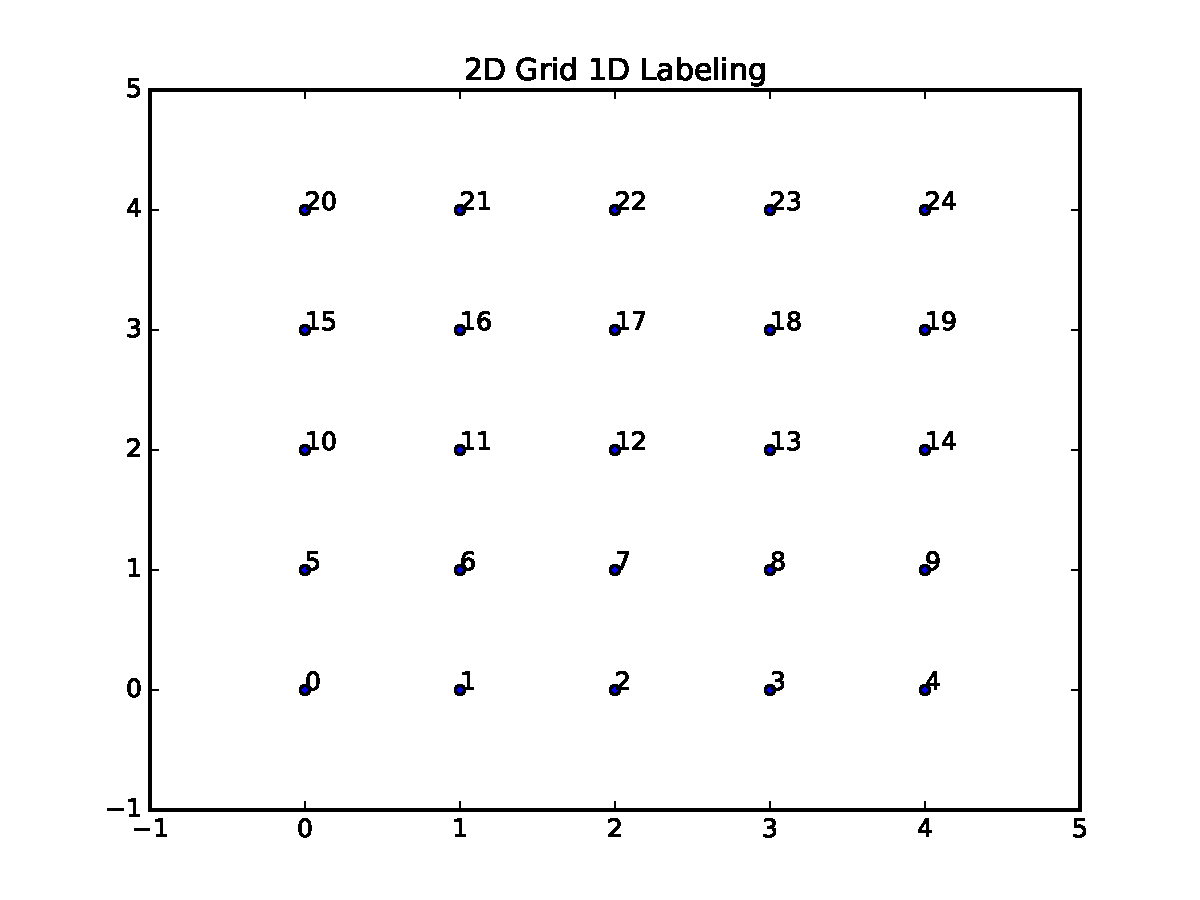
\includegraphics[width=\linewidth]{compress.pdf}
	\caption{Illustration of the compression/decompression technique for a 2 dimensional lattice. }
	\label{fig:cantor}
\end{figure*}
Figure \ref{fig:cantor} illustrates the Cantor compression scheme. The $(x,y)$ position of each point on the lattice is a 2-tuple, while the integer displayed above each point provides a unique 1-tuple label.

\section{Sanity Check}
In this section we provide basic checks that our code works. First we show using the Wolff algorithm that we find the correct critical temperatures for the dimensions referenced in the table at the beginning of the paper. We use 10 points per dimension in the following plots.

\begin{figure*}[htb!]
	\centering 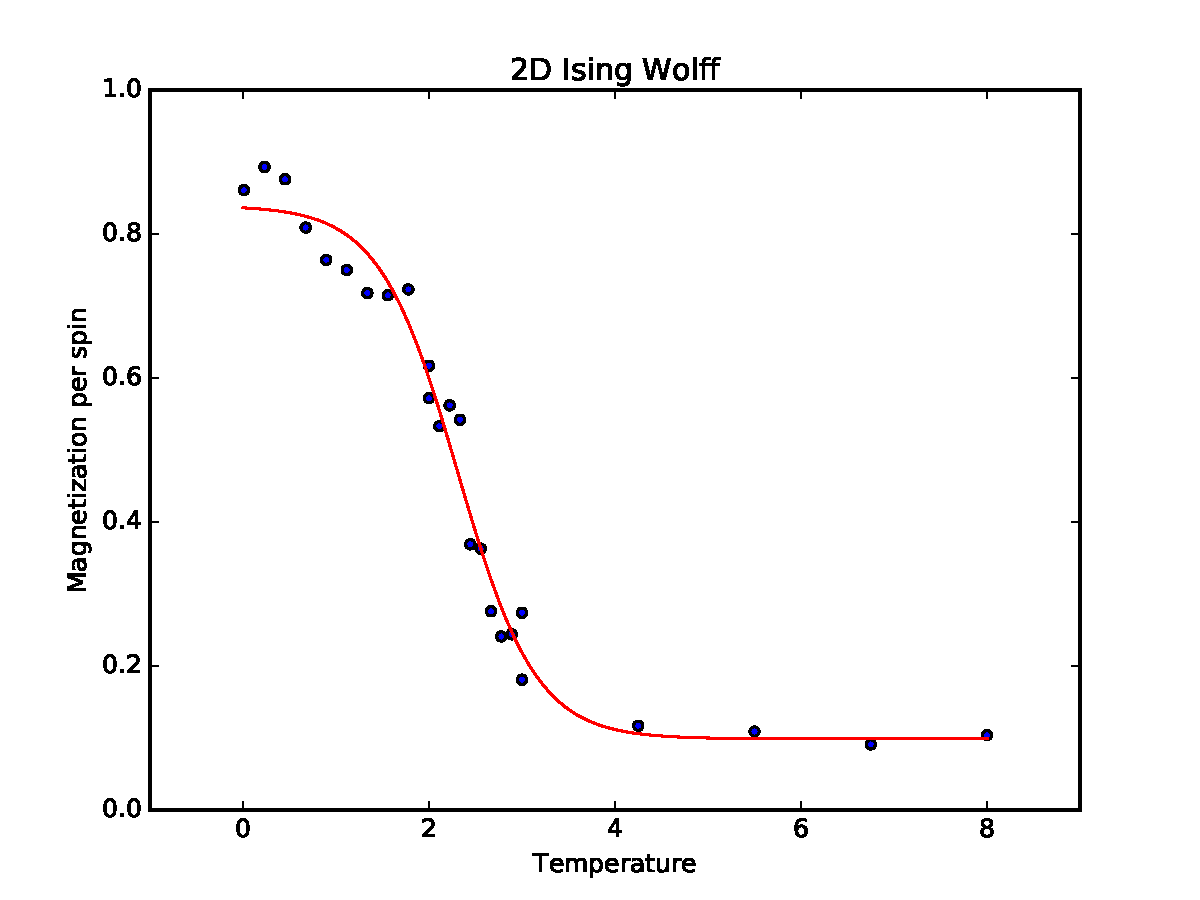
\includegraphics[width=\linewidth]{2D_Wolff.pdf}
	\caption{Plot showing the expectation value of the absolute value of the Magnetization per spin on a 2D lattice. The red line is a least squares fitted logistic function.}
	\label{fig:wolff2}
\end{figure*}

Figure \ref{fig:wolff2} shows the expected absolute magnetization per spin in the 2D Ising model. The red line shows the logistic function fit which takes the form...
\begin{center}
	$f(T)=A+\frac{K-A}{(1+Q\exp(-B(T-M)))}$
\end{center}
which we can use to analytically find the inflection point, $T_{c}$, by differentiating twice...
\begin{center}
	$T_{c}=\frac{BM-\log\left(\frac{1}{Q}\right)}{B}$
\end{center}

Using this, for 2D we find that $T_{c}=2.27$, which exactly matches the true value. We obtain similar plots for the Metropolis and Swendsen-Wang algorithms, so we are confident that the \texttt{Ising} package correctly handles 2 dimensional Ising models.

\begin{figure*}[htb!]
	\centering 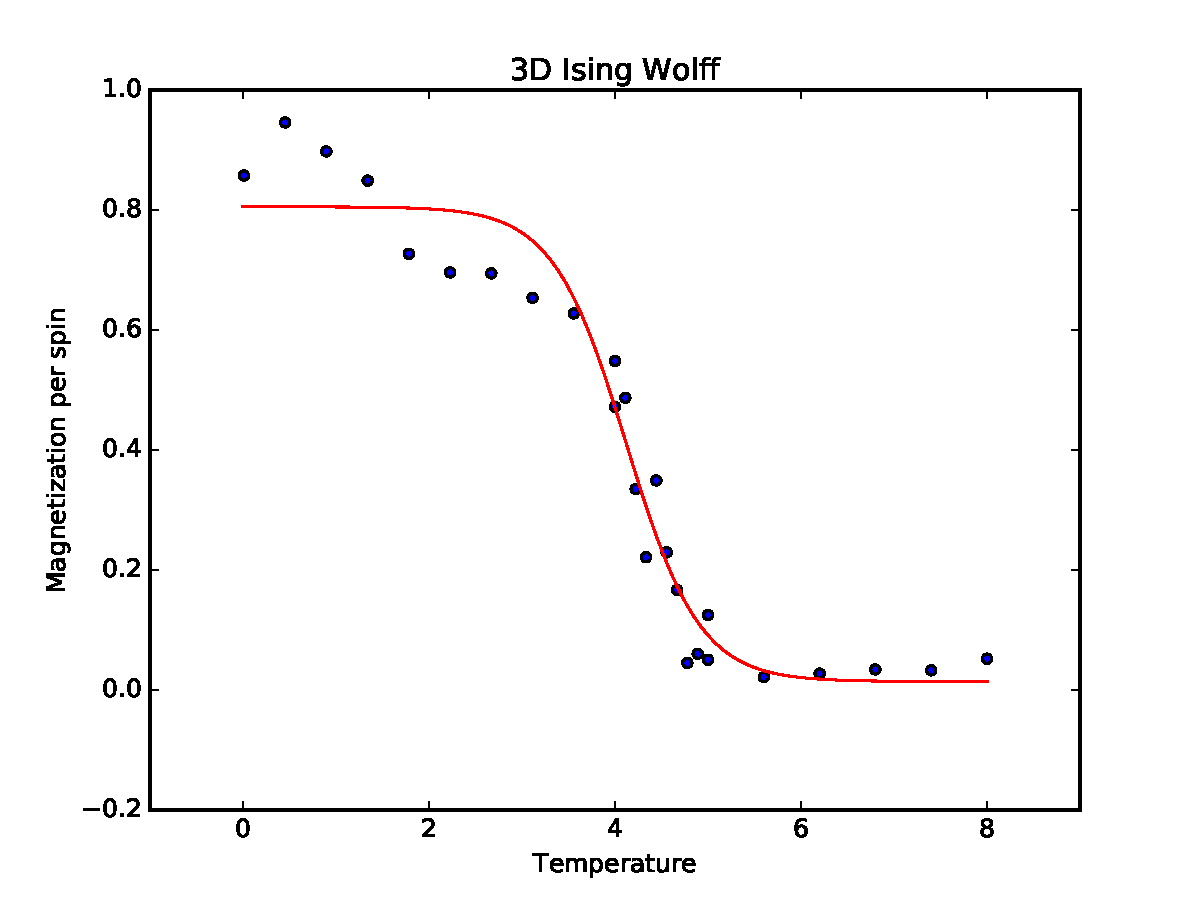
\includegraphics[width=\linewidth]{3D_Wolff.pdf}
	\caption{Plot showing the expectation value of the absolute value of the Magnetization per spin on a 3D lattice. The red line is a least squares fitted logistic function.}
	\label{fig:wolff3}
\end{figure*}

Figure \ref{fig:wolff3} shows a plot of the expected absolute magnetization per spin of the 3 dimensional Ising model. In this case, we see that the critical temperature has increased, as expected. Using the logistic fit and the analytic expression for the inflection point, we find that $T_{c}=4.3$, which is quite close to the expected result of 4.51. 


\end{document}